\section{Model Exercise 3-3 (09): Cycling loading pressure diffusion}
\label{sec:mex09}
\index{cycling loading pressure diffusion}%------------------------------------------------------------------------------
\Authors{Patrick Schmidt, Keita Yoshioka, Holger Steeb et al.}
%------------------------------------------------------------------------------
\subsection{Experimental set-up}
%------------------------------------------------------------------------------
\todo[inline]{[UoS]: Please briefly describe/refer experimental set-up}
%------------------------------------------------------------------------------
\subsection{Model approach}
%------------------------------------------------------------------------------
\subsubsection*{Finite element approach: hybrid-dimensional formulation}
A physically sound flow model assuming compressible and viscous fluids in a deformable fracture setting is used to investigate pressure diffusion within fluid-filled fractures. In order to capture local and non-local transient effects a consistent implicit coupling of both domains is necessary to guarantee stability and accuracy. Calculations on non-conformal meshes and two different computational domains motivates a so-called weak coupling scheme implemented in FENICS. A robust numerically scheme is obtained by strongly coupled interface elements implemented in the DUNE framework. 
\subsubsection*{Evaluation of strong and weak coupling scheme}
Implementation of both schemes are firstly evaluated for a single fracture under linear conditions and compared with a reference solution obtained by Biot's formulation. The weak coupling scheme is implemented using a fixed-stress and fixed-strain algorithm providing a physical preconditioning and is mathematically similar to a Richardson type iteration. The system becomes numerically stiff for low fluid compressibilities on a local level since the physics are similar to volumetrically coupled problems. Strong and weak coupling schemes are tested on a single fracture with a length of $100 \, \text{m}$ under a constant fluid pressure of $20 \, \text{kPa}$ with regards of accuracy and stability. 
\index{HDF - model validation}%------
\begin{table*}[htb]
\centering
\begin{adjustbox}{max width=\textwidth}
%\begin{adjustbox}{angle=90}
\begin{tabular}{llllll}\hline
\rule[1.9ex]{0ex}{1ex}\bf{Quantity} & \bf{Value} & \bf{Unit} & \bf{Quantity} & \bf{Value} & \bf{Unit} \\[1.1ex]\hline
\textbf{\textit{Poroelastic domain $\mathcal{B}^{Pe}$}} &&&&&  \\
intrinsic permeability $k^\mathfrak{s}$ & $1.1\cdot10^{-19}$ & [$m^2$] & min fluid comp. $\beta^f_{min}$  & $4.5\cdot10^{-10}$ & [1/Pa]  \\
max fluid comp. $\beta^f_{max}$  & $4.5\cdot10^{-4}  $ & [1/Pa] & 
sample length $l_{{Pe}}$ & $1.0\cdot10^3$ & [m] \\ 
sample height $h_{{Pe}}$ & $5.0 \cdot 10^2$ & [m] &&&\\
\textbf{\textit{Fracture domain $\mathcal{B}^{{Fr}}$}} &&&&&  \\
min fluid comp. $\beta^f_{min}$  & $4.5\cdot10^{-10} $ & [1/Pa] & max fluid comp. $\beta^f_{max}$  & $4.5\cdot10^{-4}  $ & [1/Pa] \\ 
fracture aperture $\delta_0$ & $5.0\cdot10^{-3}$ & [m] & fracture length $l^{Fr}$ & $1.0 \cdot 10^2$ & [m] \\
pumping pressure $p_0$ & $2.0\cdot10^4$ & [Pa] &  &  & \\
\textbf{\textit{Numerical Parameter}} &&&&&  \\
time step size $\Delta t$ & $1.0\cdot10^{-2}$ & [s] &
fracture discret. in $\mathcal{B}^{Fr}$ $\Delta x^{Fr}_{Fr}$ & $1.0\cdot10^{-1}$ & [m] \\
fracture discret. in $\mathcal{B}^{Pe}$ $\Delta x^{Fr}_{Pe}$ & $1.0\cdot10^{-1}$ & [m] &
evaluation time $t_0$ & $1.0 \cdot 10^1$ & [s] \\
evaluation position $x_0$ & $1.0 \cdot 10^1$ & [m] & error tolerance $\epsilon_{max}$ & $1.0 \cdot 10^{-6}$ & [-] \\
number of DoF & $1.4 \cdot 10^5$ & [-]& & & \\
\hline
\end{tabular}
\end{adjustbox}
\caption{Collection of parameters used for validation of the weak and strong coupling schemes.}
\label{tab:validationparameters}
\end{table*}

\begin{figure}[!ht]
\centering
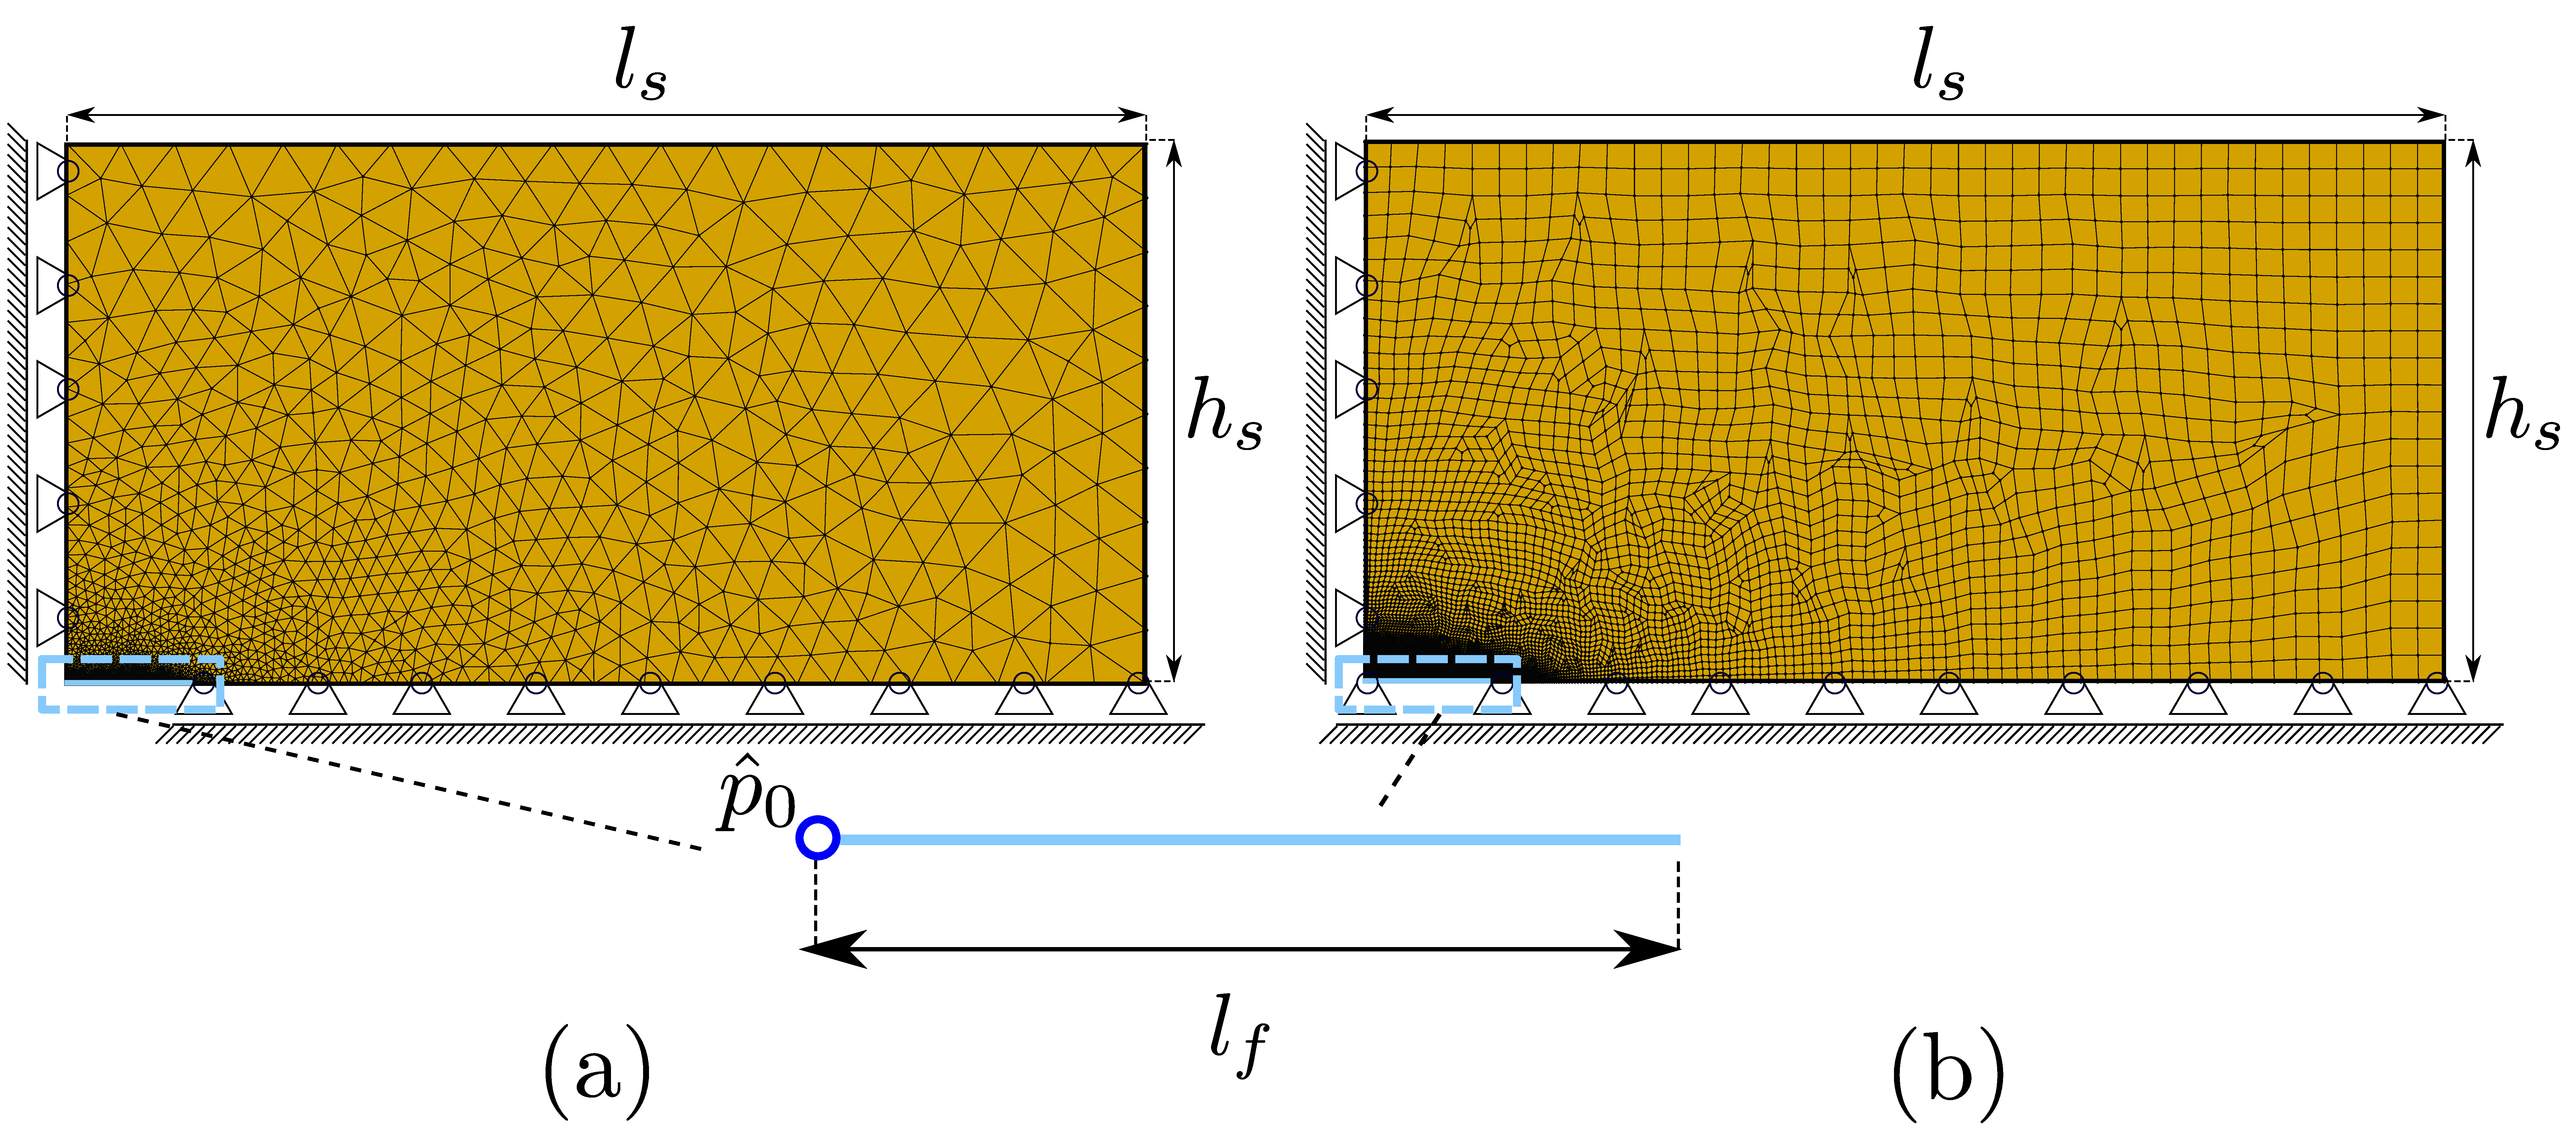
\includegraphics[width=1\linewidth]{figures/ME9_benchmark_set_up.pdf}
\caption{Discretization and boundary conditions used for the weak coupling (a) and strong coupling scheme
(b) throughout the validation.}
\label{fig:ME9_validation_set_up}
\end{figure}
\begin{figure}
\centering
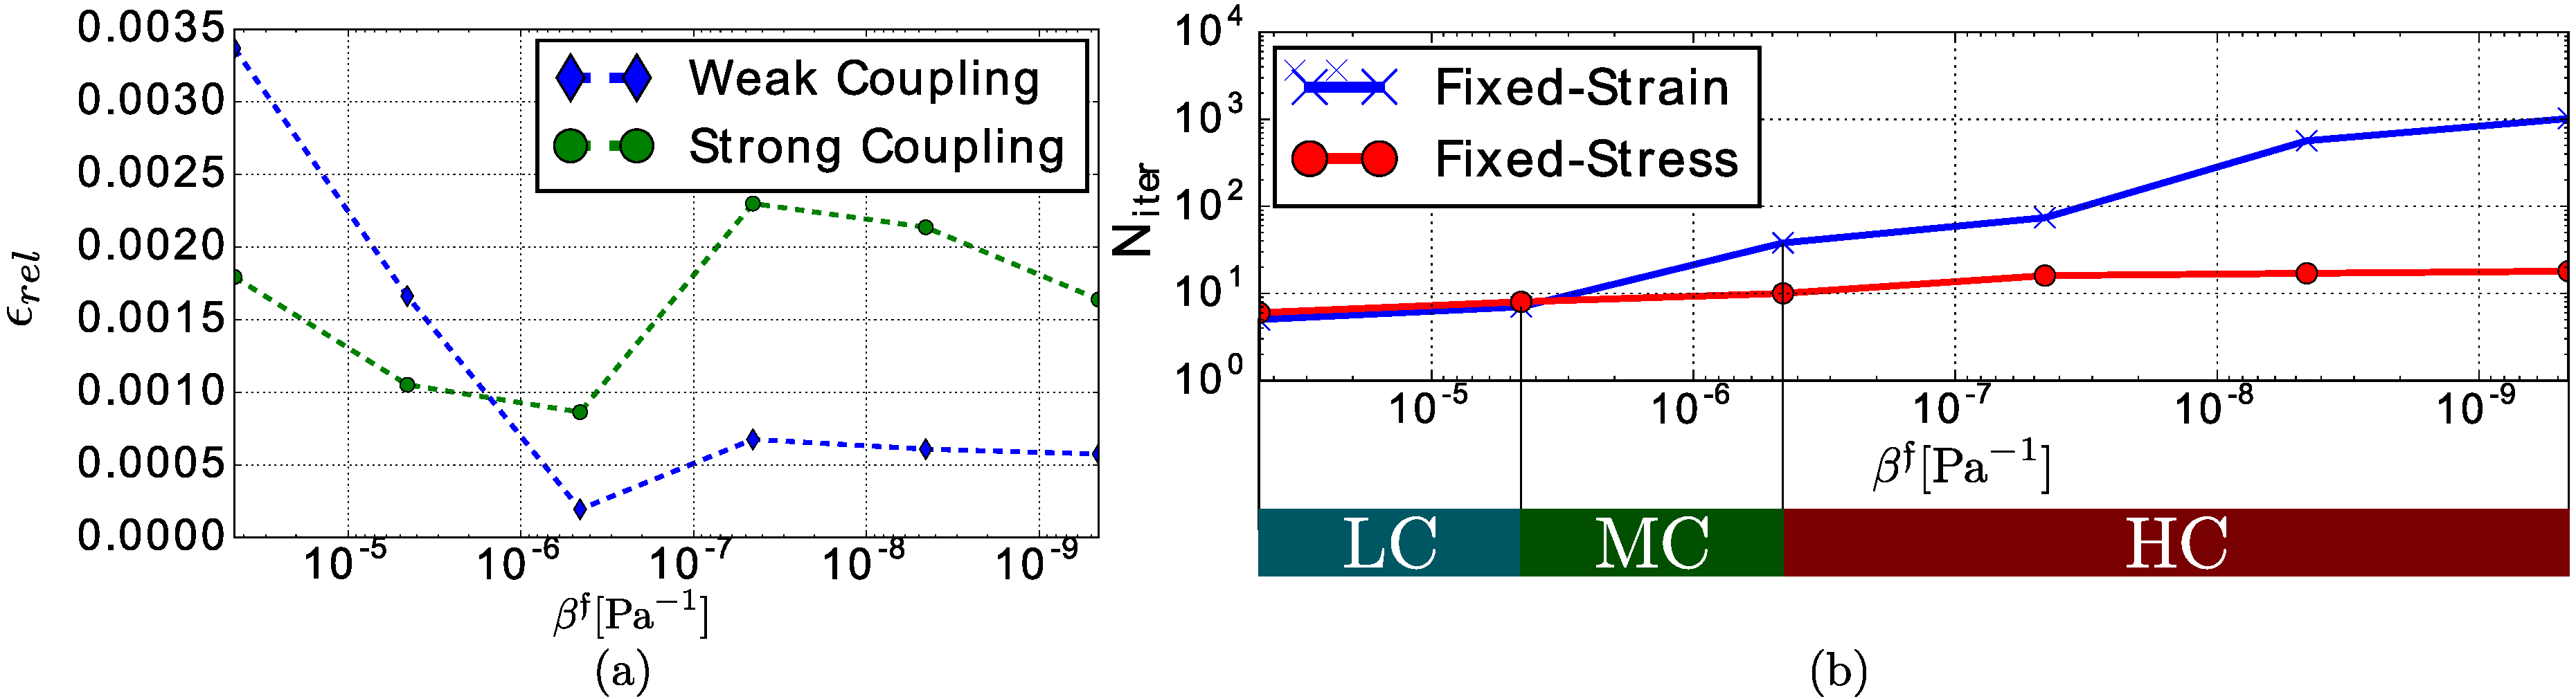
\includegraphics[width=1\linewidth]{figures/ME9_compressibility_study.pdf}
\caption{Plot of the relative error $\epsilon_{rel}$ for the strong and weak coupling schemes (a) and recommended compressibility range of application for both methods based on the necessary number of iterations $N_{iter}$ of the fixed-strain and fixed-stress scheme for \textbf{L}ow \textbf{C}ompressibilities, \textbf{M}oderate \textbf{C}ompressibilities and \textbf{H}igh \textbf{C}ompressibilities of the fluid (b).}
\label{fig:ME9_validation_compressibility}
\end{figure}

\subsubsection*{Non-Linear Evaluation}
Large deformations in high aspect ratios are reached for small absolute deformation values already and highly influences the fracture flow by local (permeability) and non-local (volumetric) deformation related perturbations. Time dependent pressure/flow stimulation requires a continuous transient change of fracture aperture and deformation dependent pressure diffusion. Validation of the non-linear formulation is using a cylindrical probe with a single fracture under a confining pressure $\sigma_c$ and a harmonic pressure stimulation $p(t)$. In order to study the behaviour the amplitude of stimulation pressure is increased to enforce large deformation changes within a period.
\index{non-linear pressure-flux relation}%------

\begin{table*}[htb]
\centering
\begin{adjustbox}{angle=90}%{max width=\textwidth}
\begin{tabular}{llllll}\hline
\rule[1.9ex]{0ex}{1ex}\bf{Quantity} & \bf{Value} & \bf{Unit} & \bf{Quantity} & \bf{Value} & \bf{Unit} \\[1.1ex]\hline
\textbf{\textit{Rock matrix}} &&&&&  \\
dry frame bulk modulus $K$ & $2.2 \cdot 10^{10}$ & [Pa] & grain bulk modulus $K^\mathfrak{s}$ & $4.6\cdot 10^{10}$ & [Pa] \\
shear modulus $\mu$ & $1.77 \cdot 10^{10}$ & [Pa] & porosity $\phi$ & $1.0\cdot10^{-2}$ & [-]  \\
intrinsic permeability $k^\mathfrak{s}$ & $5.0 \cdot 10^{-19}$  & [$\text{m}^2$] &  
fluid compressibility $\beta^f$  & $4.17 \cdot 10^{-10}$  & [1/Pa] \\
effective bulk modulus $K_{eff}$ & $3.98 \cdot 10^{10}$  & [Pa] &  effective shear modulus $\mu_{eff}$  
& $1.77 \cdot 10^{10}$  & [Pa] \\
\textbf{\textit{Fracture domain}} &&&&&  \\
effective fluid viscosity $\eta^{\mathfrak{f}R}$ & $1.0\cdot10^{-3}$ & [Pa$\cdot$s] & 
initial fracture aperture $\delta_0$ & $2.5 \cdot 10^{-6}$ & [m]\\
equilibrium fracture aperture $\delta_{eq}$ & $4.61 \cdot 10^{-6}$ & [m] &  
fluid compressibility $\beta^f$  & $4.17 \cdot 10^{-10}$  & [1/Pa] \\
\multicolumn{5}{l}{\textbf{\textit{Sample Geometry and Hydraulic Stimulation}}}  \\
sample height $h$ & $7.5\cdot10^{-2}$ & [m] &
sample diameter $d$ & $3.0\cdot10^{-2}$ & [m] \\
borehole diameter $d_b$ & $6.0\cdot10^{-3}$ & [m] &
stimulation period $T$ & $2.0\cdot \pi$ & [sec] \\
equilibrium pressure $p_{eq}$ & $1.5\cdot10^{7}$ & [Pa] &
reference Amplitude $p_A^{lin}$ & $1.0\cdot10^{3}$ & [Pa] \\
minimum Amplitude $p_{A}^{min}$ & $0.5\cdot10^{6}$ & [Pa] &
maximum Amplitude $p_{A}^{max}$ & $3.0\cdot10^{6}$ & [Pa] \\
pressure increment $\Delta p_{A}$ & $0.5\cdot10^{6}$ & [Pa] &
confining pressure $p_{c}$ & $2.0\cdot10^{7}$ & [Pa] \\
\hline
\end{tabular}
\end{adjustbox}
\caption{Collection of parameters used throughout numerical periodic hydraulic stimulation experiment on a sandstone probe.}
\label{tab:non_conformal_parameters}
\end{table*}

\begin{figure}
\centering
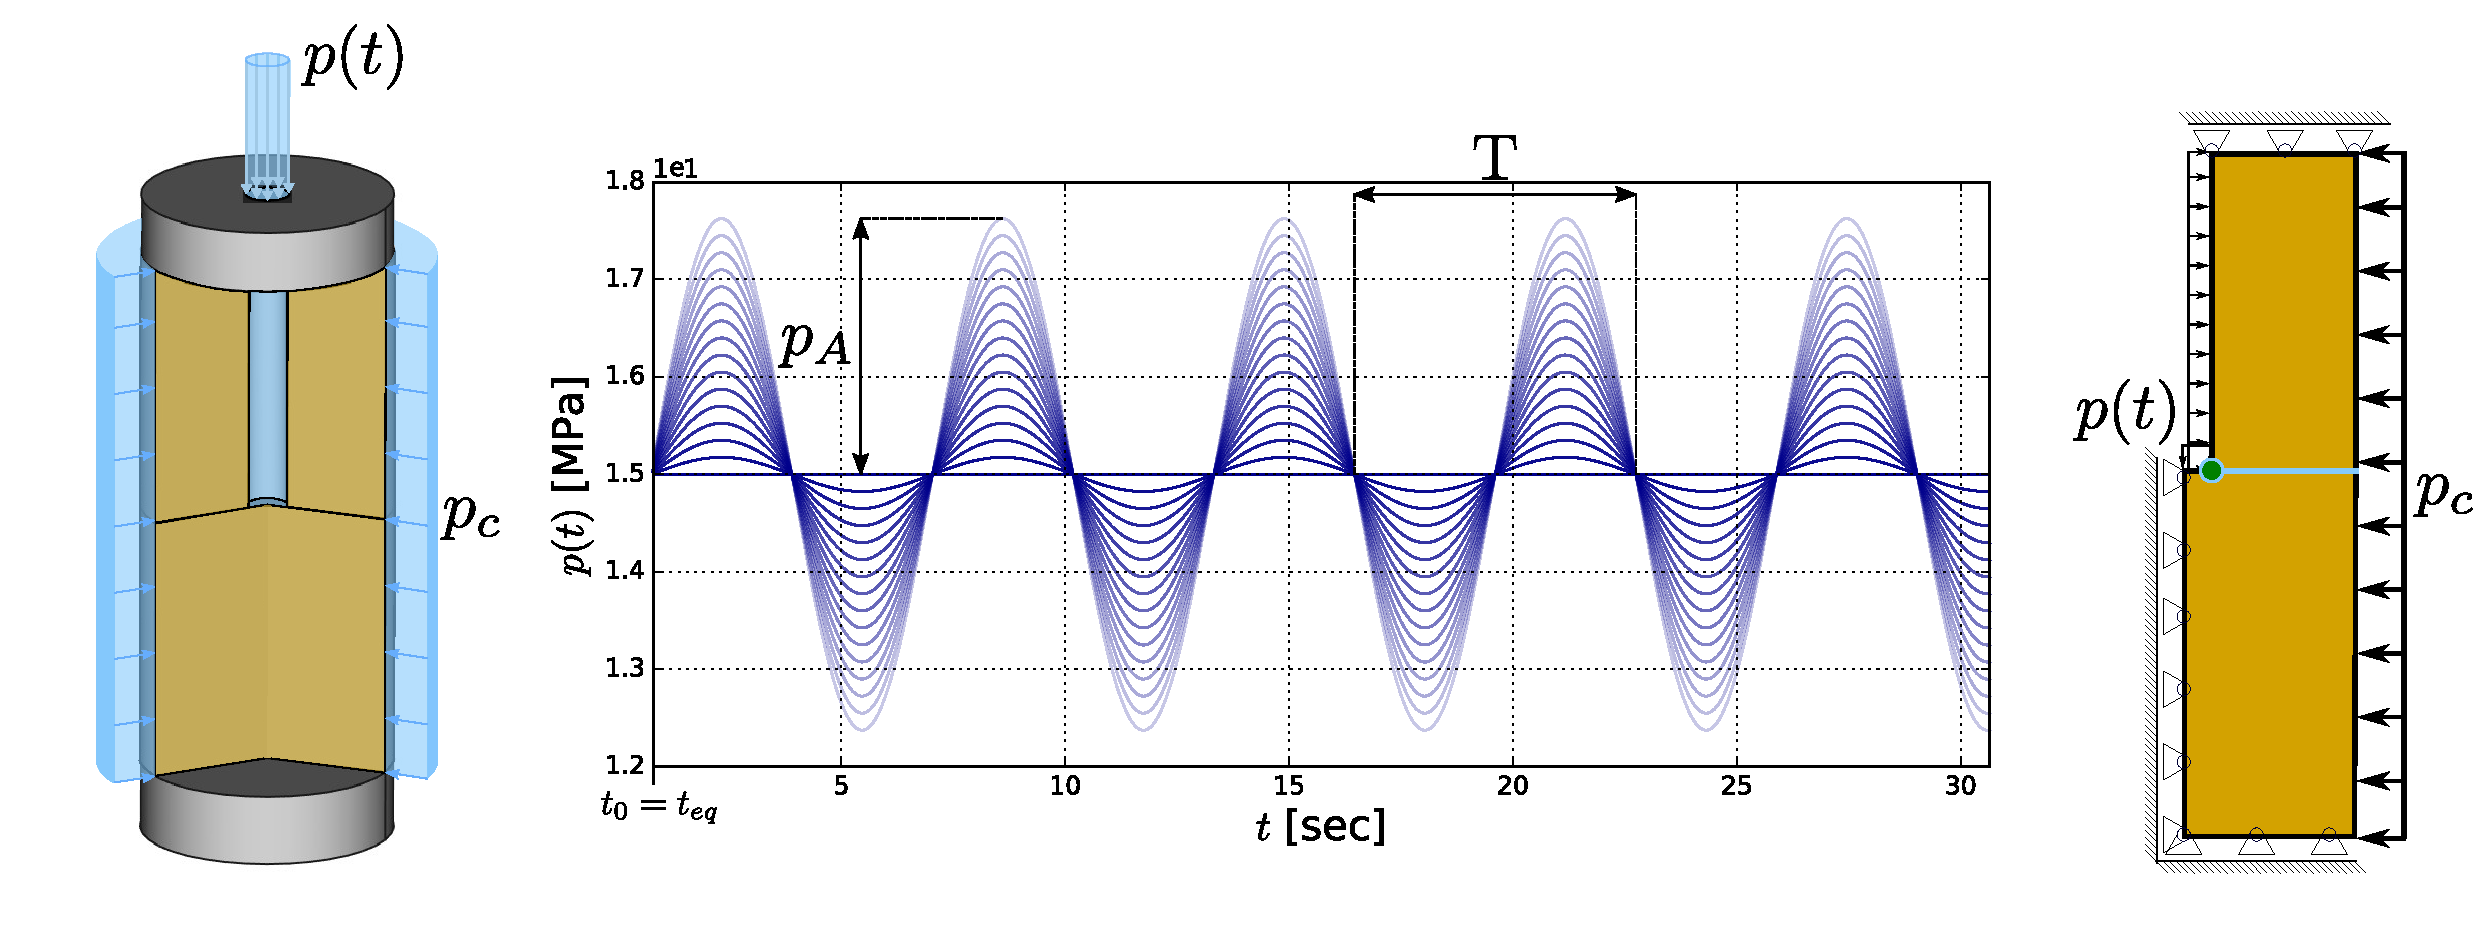
\includegraphics[width=1\linewidth]{figures/ME9_experimental_set_up_nl_pq.pdf}
\caption{Numerical set up of cylindrical probe under periodic hydraulic pressure $p(t)$ and
confining pressure $p_c$.}
\label{fig:ME9_validation_set_up1}
\end{figure}
\begin{figure}
\centering
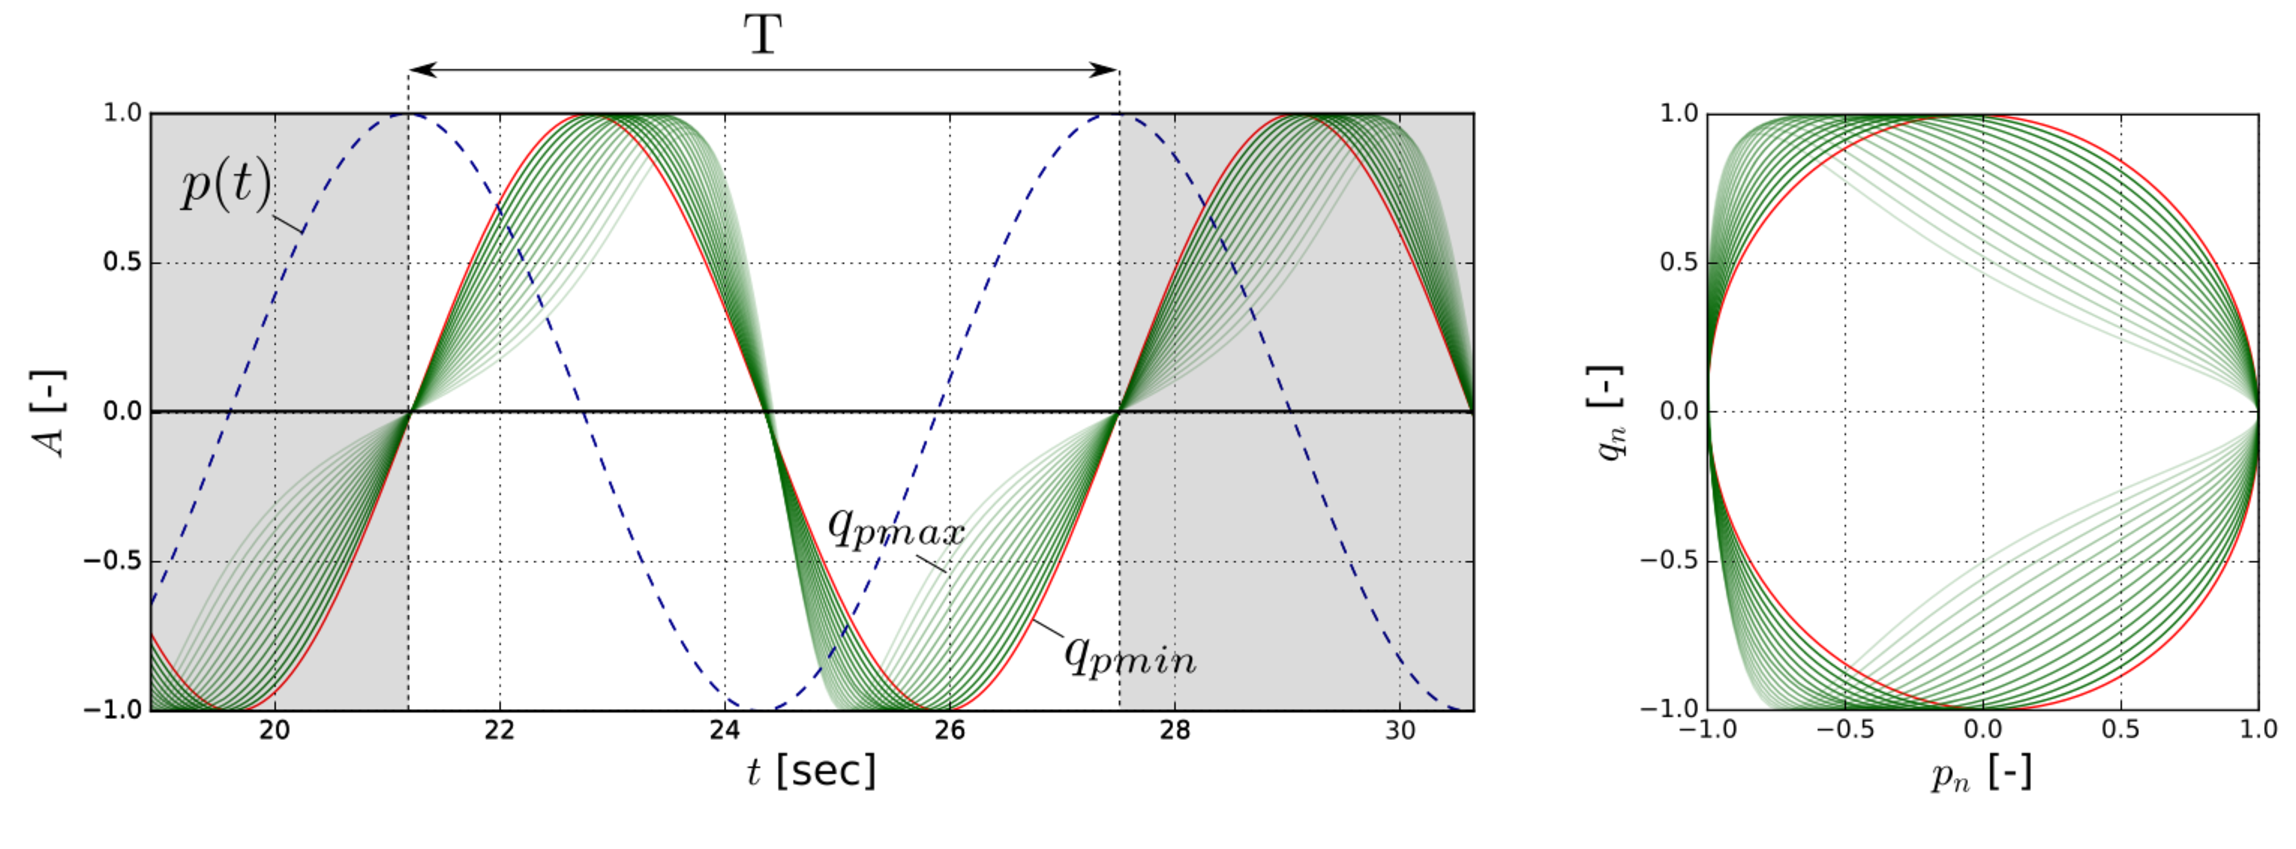
\includegraphics[width=1\linewidth]{figures/ME9_non_linear_p_q.pdf}
\caption{Presentation of $p-q$ comparison via time and hysteresis plot. Flux solutions $q_n$ are
highlighted in green scales for varying pressure amplitudes normalized with respect to its maximum value, the normalized linear flux solution $q_{lin}$ is highlighted in red and the normalized stimulation pressure $p_n(t)$ is highlighted in blue.}
\label{fig:ME9_validation_compressibility1}
\end{figure}

\subsubsection*{Model by variational phase-field model}
The variational phase-field implementation in OGS is tested under the same condition.
Crack opening in the variational phase-field mode is not direct variable but is a reconstruction from the diffused variables~\cite{Yoshioka2020}.
The axisymmetric model with the same settings is prepared as shown in~\ref{fig:ME3-3_pressrue_VPF_init}.

\begin{figure}
\centering
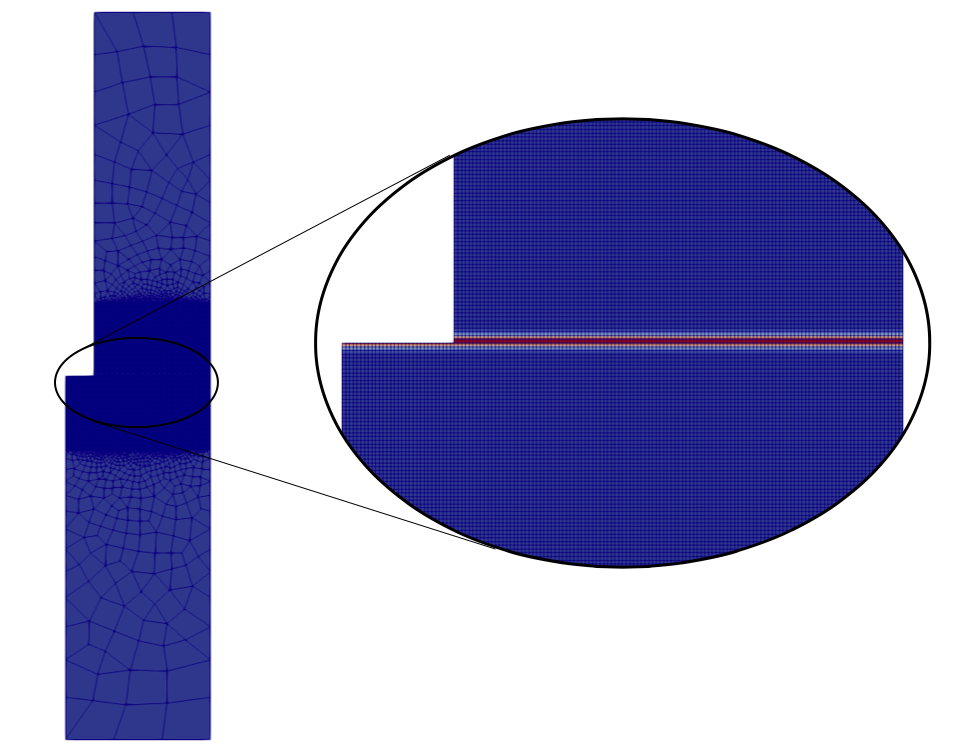
\includegraphics[width=1\linewidth]{figures/VPF_ME3-3_init.png}
\caption{Finite element mesh set up for aariational phase-field simulation.}
\label{fig:ME3-3_pressrue_VPF_init}
\end{figure}

\begin{figure}
\centering
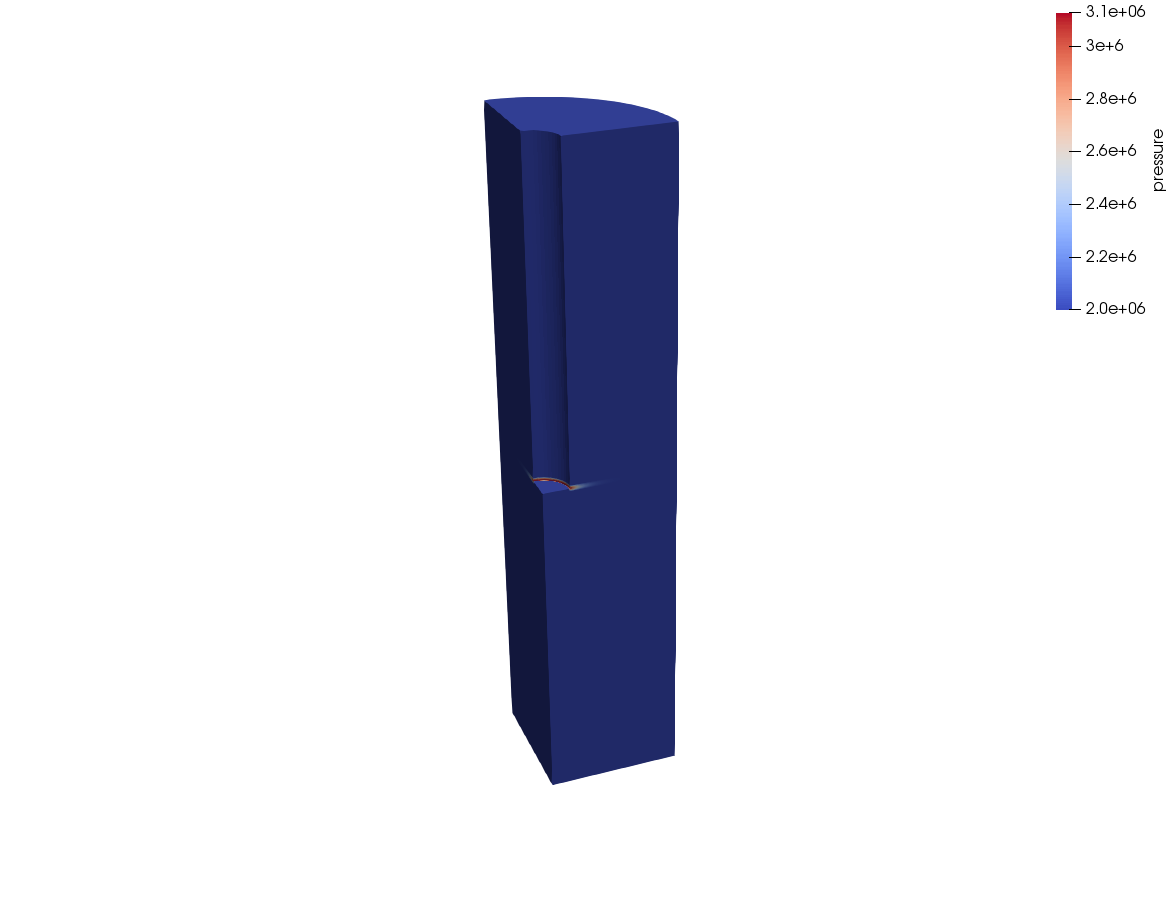
\includegraphics[width=1\linewidth]{figures/Keita_ME9_pres.png}
\caption{Pressure simulation from the variational phase-field.}
\label{fig:ME9_pressrue_VPF}
\end{figure}
\begin{figure}
\centering
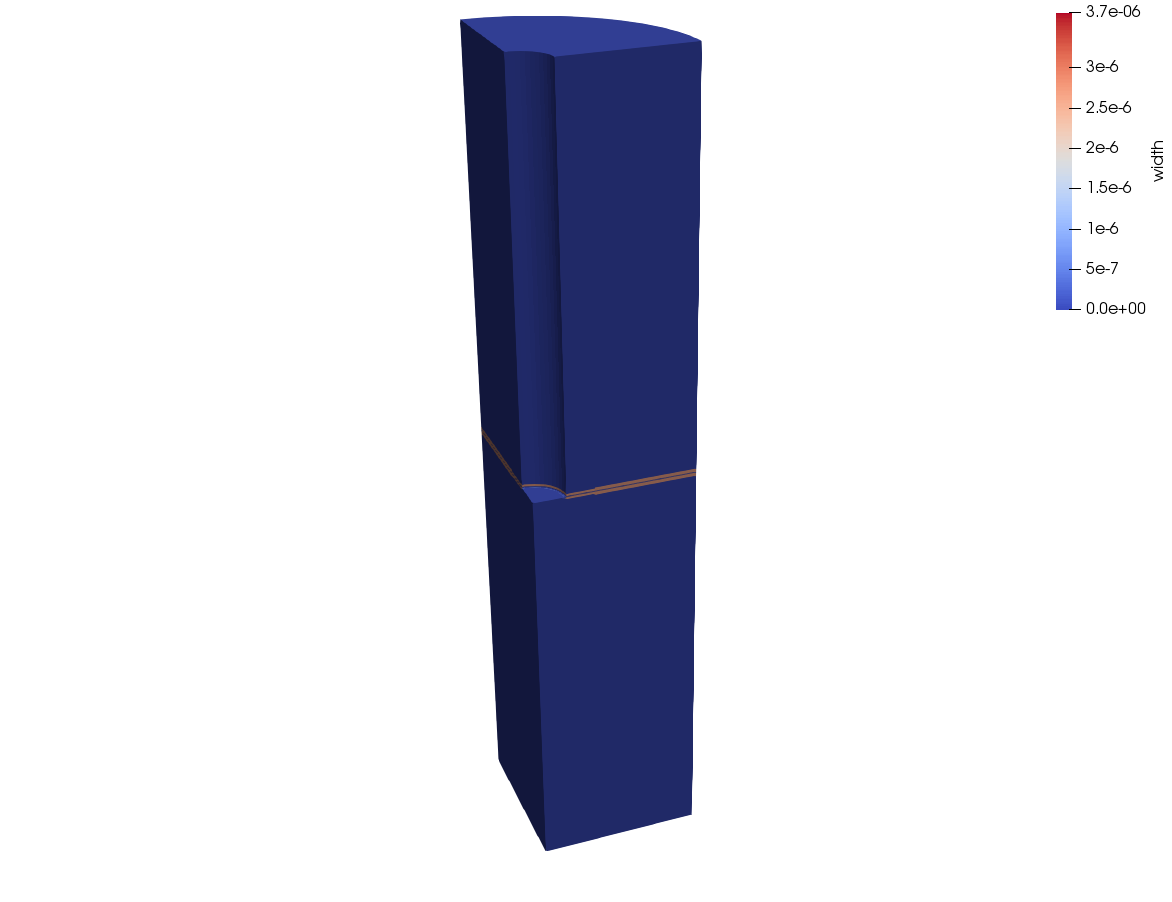
\includegraphics[width=1\linewidth]{figures/Keita_ME9_width.png}
\caption{Crack opening from the variational phase-field.}
\label{fig:ME9_width_VPF}
\end{figure}

\todo[inline]{[UFZ] Keita: Please extend the VPF discussion a bit}

%------------------------------------------------------------------------------
\subsection{Results and discussion}
Harmonic, fluid pressure induced perturbations of the fracture's equilibrium state result in a non-linear pressure-flow ($p-q$) relationship as shown in Fig. \ref{fig:ME9_validation_compressibility1}. Injected fluid volume results in a volume change of the fracture leading to non-constant permeabilities throughout a testing period and changes of the characteristic diffusion time of the investigated system. The effect scales with the magnitude of the applied pressure amplitude since deformations of the fracture and changes in permeability are responses of the system to the non-constant acting pressure conditions. The phenomenon of non-linear pressure flow ($p-q$) relations emphasizes the importance of characteristic changes due to induced deformations of investigated fractures and might serve as a tool to characterize the transient volume change.
